\begin{figure}
	\centering
	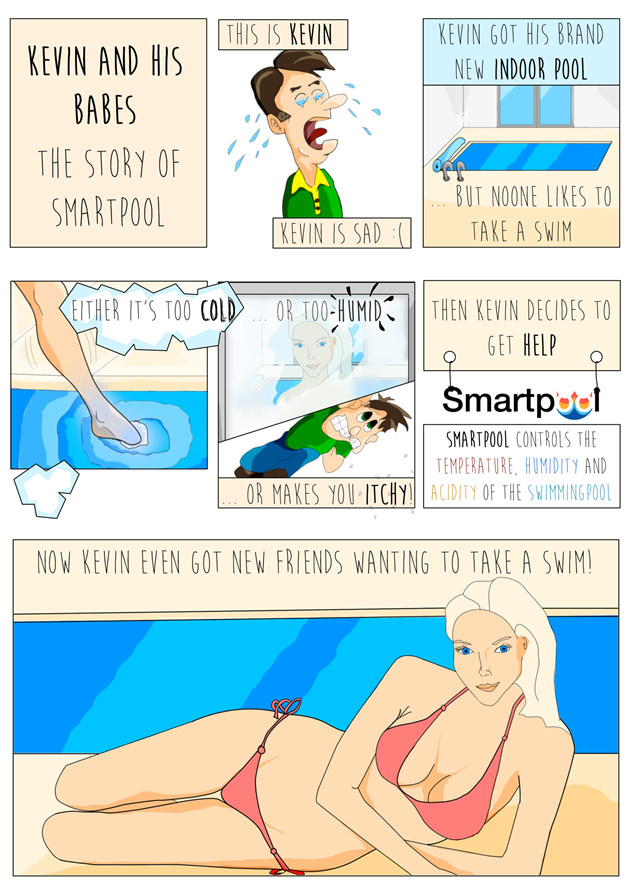
\includegraphics[width=0.99\linewidth]{figs/kevin.png}
	\label{fig:kevin}
\end{figure}

\newpage

\section{Projektformulering}
Smartpool er et system, som kan måle bestemte forhold for en swimmingpool. 
Det er forhold som:
\begin{itemize}
	\item Temperatur.
	\item pH-værdi.
	\item Klorindhold.
\end{itemize}

Er der tale om en indendørspool fås en speciel udgave, som også kan måleluftfugtighed i det indendørspool rum.

Smartpool måler forholdene vha. sensorer. Sensorerne måler forholdene for vandet eller luften omkring poolen. Målinger distribueres via. Smartpool systemet til en database. Brugeren af Smartpool kan tilgå databasen vha. En webapplikation eller anden form for app. 

Brugeren kan derved monitorerer forholdene og derved opnå et bedre pool klima. Brugeren behøver ikke være på et lokalt netværk, blot brugeren har adgang til internettet, kan Smartpools applikationer vise pool forhold og historik. 

Smartpools fjerndistance egenskab er særlig anvendelig for sommerhusejere, som udlejer sommerhuset. Der er visse krav til en pool, som skal overholdes i forbindelse med udleje. Smartpool hjælper med vedligeholdelsen af poolen, ved at notificere brugeren om, at poolen ikke overholder acceptable forhold. 

Mindst en gang ugentlig skal der i pool foretages målinger for indholdet af frit og bundet klor samt pH i henhold til gældende reglement.

Smartpool vil da hjælpe brugeren med anbefalet dosering af kemikalier eller påmindelse om at starte opvarmning af poolen.

Smartpool erstatter termometer, pH-papir og klortester. For indendørspool også hydrometer. Smartpools notifikationsfunktion kan erstatte en tilsynsfører. Brugeren kan dermed nemmere selv styre pool forholdene, hvormed brugeren ikke behøver at have poolen i udlejningsbureau.
